%%%%%%%%%%%%%%%%%%%%%%%%%%%%%%%%%%%%%%%%%%%%%%%%%%%%%%%%%%%%%%%%%%%%%%
% Overleaf (WriteLaTeX) Example: Molecular Chemistry Presentation
%
% Source: http://www.overleaf.com
%
% In these slides we show how Overleaf can be used with standard 
% chemistry packages to easily create professional presentations.
% 
% Feel free to distribute this example, but please keep the referral
% to overleaf.com
% 
%%%%%%%%%%%%%%%%%%%%%%%%%%%%%%%%%%%%%%%%%%%%%%%%%%%%%%%%%%%%%%%%%%%%%%

\documentclass{beamer}

\mode<presentation>
{
  \usetheme{Madrid}       % or try default, Darmstadt, Warsaw, ...
  \usecolortheme{default} % or try albatross, beaver, crane, ...
  \usefonttheme{default}    % or try default, structurebold, ...
  \setbeamertemplate{navigation symbols}{}
  \setbeamertemplate{caption}[numbered]
} 

\usepackage[english]{babel}
\usepackage[utf8x]{inputenc}
\usepackage{chemfig}
\usepackage[version=3]{mhchem}

\usepackage{hyperref}
  \hypersetup{colorlinks=true}
  \hypersetup{urlcolor=blue}
  \hypersetup{linkcolor = .}
\usepackage{xcolor}
\usepackage{siunitx}
  \sisetup{separate-uncertainty = true}
\usepackage{physics}
\usepackage[font=small,labelfont=bf]{caption}
\usepackage{subcaption}
\usepackage[en-GB]{datetime2}
\usepackage{overpic}
\usepackage{feynmp}
\DeclareGraphicsRule{*}{mps}{*}{}

\usepackage{scalerel}
\newcommand{\mylbrace}[2]{\vspace{#2pt}\hspace{6pt}\scaleleftright[\dimexpr5pt+#1\dimexpr0.06pt]{\lbrace}{\rule[\dimexpr2pt-#1\dimexpr0.5pt]{-4pt}{#1pt}}{.}}
\newcommand{\myrbrace}[2]{\vspace{#2pt}\scaleleftright[\dimexpr5pt+#1\dimexpr0.06pt]{.}{\rule[\dimexpr2pt-#1\dimexpr0.5pt]{-4pt}{#1pt}}{\rbrace}\hspace{6pt}}

% Here's where the presentation starts, with the info for the title slide
\title[$B^\pm\to(K^+K^-\pi^+\pi^-)_DK^\pm$]{CKM angle \texorpdfstring{$\gamma$}{gamma} determination in \texorpdfstring{$B^\pm\to DK^\pm$, $D\to K^+K^-\pi^+\pi^-$}{B to DK, D to K+K-pi+pi-} decays}
\author{Martin Tat}
\institute{Oxford LHCb}
\date{22nd June 2021}

\titlegraphic{\includegraphics[height = 3cm, width = 4cm]{lhcb.jpg}\hspace{2cm}~%
              \includegraphics[height = 3cm, width = 4cm]{ckmfitter.png}}

\begin{document}

\begin{frame}
  \titlepage
\end{frame}

% These three lines create an automatically generated table of contents.
\begin{frame}{Outline}
  \tableofcontents
\end{frame}

\section{\texorpdfstring{$\gamma$}{gamma} and the unitary triangle}
\begin{frame}{$\gamma$ and the unitary triangle}
  \begin{center}
    {\huge $\gamma$ and the unitary triangle} \\
    \vspace{1cm}
    {\Large How to measure $\gamma$?}
  \end{center}
\end{frame}

\begin{frame}{$\gamma$ and the unitary triangle}
  \begin{itemize}
    \setlength\itemsep{1.0em}
    \item{Unitarity of CKM matrix: $V_{ud}V^*_{ub} + V_{cd}V^*_{cb} + V_{td}V^*_{tb} = 0$}
    \item{Define $\gamma = \text{arg}\Big(-\frac{V_{ud}V^*_{ub}}{V_{cd}V^*_{cb}}\Big)$}
    \item{Only CKM angle accessible at tree level $\implies$}
    \begin{itemize}
      \item{Negligible theoretical uncertainties}
      \item{Ideal Standard Model benchmark}
    \end{itemize}
  \end{itemize}
  \vspace{-0.2cm}
  \begin{figure}
    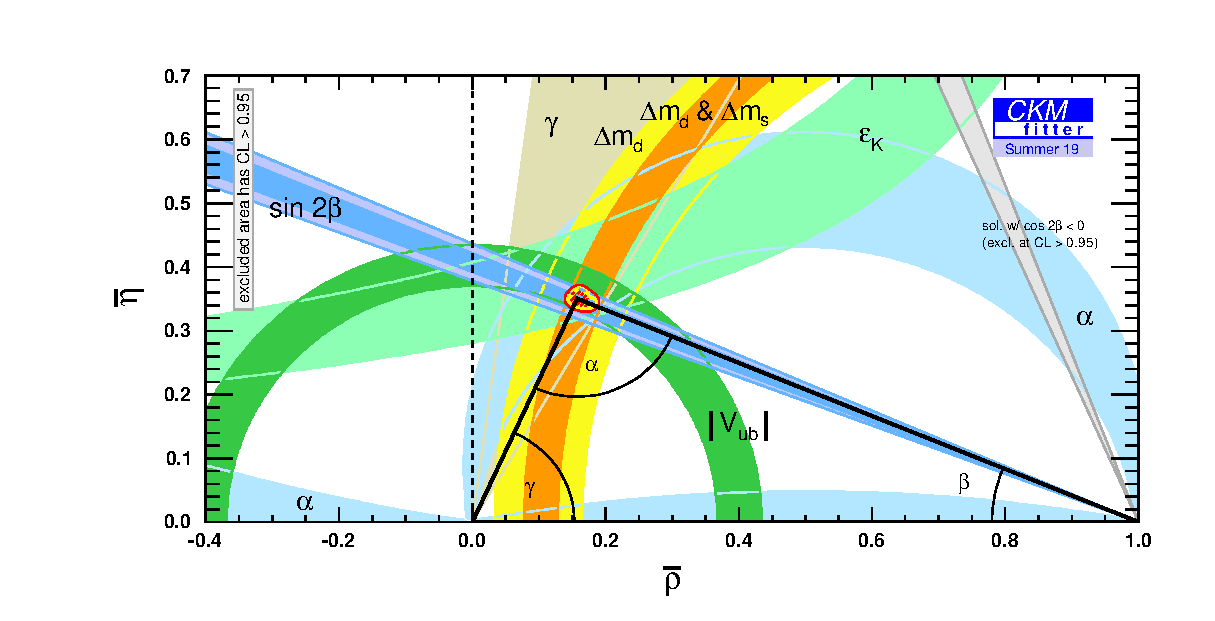
\includegraphics[width = 0.70\textwidth]{ckmfitter2.eps}
  \end{figure}
  \vspace{-0.7cm}
  \begin{center}
    CKMfitter Group (J. Charles et al.), Eur. Phys. J. C41, 1-131 (2005)
  \end{center}
\end{frame}

\begin{frame}{How to measure $\gamma$?}
  \begin{figure}[H]
    \centering
    \vspace{0.3cm}
    \begin{subfigure}{0.5\textwidth}
      \centering
      \begin{fmffile}{fgraph/fgraph_BtoDK1}
        \setlength{\unitlength}{0.4cm}
        \begin{fmfgraph*}(6,6)
          \fmfstraight
          \fmfleft{i1,B,i2,t1,t2,t3,t9,t10}
          \fmfright{o1,D,o2,t4,t5,o3,K,o4}
          \fmflabel{$\bar{u}$}{i1}
          \fmflabel{$b$}{i2}
          \fmfv{l.d=20,l.a=180,l={$B^-$\mylbrace{30}{-8}}}{B}
          \fmflabel{$\bar{u}$}{o1}
          \fmflabel{$c$}{o2}
          \fmflabel{$\bar{u}$}{o3}
          \fmflabel{$s$}{o4}
          \fmfv{l.d=15,l.a=0,l={\myrbrace{30}{-12}}$D^0$}{D}
          \fmfv{l.d=15,l.a=0,l={\myrbrace{30}{11}}$K^-$}{K}
          \fmf{fermion}{o1,i1}
          \fmf{fermion,tension=1.5}{i2,v1}
          \fmf{fermion}{v1,o2}
          \fmf{phantom,tension=1.5}{t9,v2}
          \fmf{boson,label=$W$,label.side=left,tension=0}{v1,v2}
          \fmf{fermion}{v2,o4}
          \fmf{fermion}{o3,v2}
        \end{fmfgraph*}
      \end{fmffile}
      \vspace{0.5cm}
      \caption{$B^-\to D^0K^-$}
    \end{subfigure}%
    \begin{subfigure}{0.5\textwidth}
      \centering
      \begin{fmffile}{fgraph/fgraph_BtoDK2}
        \setlength{\unitlength}{0.4cm}
        \begin{fmfgraph*}(6,6)
          \fmfstraight
          \fmfleft{i1,t1,t2,B,t9,t10,i2}
          \fmfright{o1,K,o2,t4,t5,o3,D,o4}
          \fmflabel{$\bar{u}$}{i1}
          \fmflabel{$b$}{i2}
          \fmfv{l.d=20,l.a=180,l={$B^-$\mylbrace{100}{-8}}}{B}
          \fmflabel{$\bar{u}$}{o1}
          \fmflabel{$s$}{o2}
          \fmflabel{$\bar{c}$}{o3}
          \fmflabel{$u$}{o4}
          \fmfv{l.d=15,l.a=0,l={\myrbrace{30}{13}}$\bar{D^0}$}{D}
          \fmfv{l.d=15,l.a=0,l={\myrbrace{30}{-13}}$K^-$}{K}
          \fmf{fermion}{o1,i1}
          \fmf{fermion,tension=1.5}{i2,v1}
          \fmf{fermion}{v1,o4}
          \fmf{phantom,tension=1.5}{t2,v2}
          \fmf{boson,label=$W$,label.side=right,tension=0}{v1,v2}
          \fmf{fermion}{v2,o2}
          \fmf{fermion}{o3,v2}
        \end{fmfgraph*}
      \end{fmffile}
      \vspace{0.5cm}
      \caption{$B^-\to\bar{D^0}K^-$ (colour suppressed)}
    \end{subfigure}
  \end{figure}
  \vspace{0.1cm}
  \begin{itemize}
    \setlength\itemsep{1.0em}
    \item{Need $b\to c\bar{u}s$ and $b\to u\bar{c}s$ interference, such as $B^\pm\to DK^\pm$}
    \begin{itemize}
      \item{$D$: Superposition of $D^0$ and $\bar{D^0}$}
    \end{itemize}
    \item{Inteference when $D^0$ and $\bar{D^0}$ decay into a common final state}
    \item{Single most precise measurement ($D\to K_S^0h^+h^-$): $\gamma = (68.7^{+5.2}_{-5.1})^\circ$ \href{https://arxiv.org/abs/2010.08483}{JHEP 02 (2021) 169}}
  \end{itemize}
\end{frame}

\begin{frame}{Simplified $\gamma$ measurement}
  \begin{figure}[H]
    \centering
    \vspace{0.3cm}
    \begin{subfigure}{0.5\textwidth}
      \centering
      \begin{fmffile}{fgraph/fgraph_BtoDK1Small}
        \setlength{\unitlength}{0.4cm}
        \begin{fmfgraph*}(5,4)
          \fmfstraight
          \fmfleft{i1,B,i2,t1,t2,t3,t9,t10}
          \fmfright{o1,D,o2,t4,t5,o3,K,o4}
          \fmflabel{$\bar{u}$}{i1}
          \fmflabel{$b$}{i2}
          \fmfv{l.d=20,l.a=180,l={$B^-$\mylbrace{30}{-8}}}{B}
          \fmflabel{$\bar{u}$}{o1}
          \fmflabel{$c$}{o2}
          \fmflabel{$\bar{u}$}{o3}
          \fmflabel{$s$}{o4}
          \fmfv{l.d=15,l.a=0,l={\myrbrace{30}{-12}}$D^0$}{D}
          \fmfv{l.d=15,l.a=0,l={\myrbrace{30}{11}}$K^-$}{K}
          \fmf{fermion}{o1,i1}
          \fmf{fermion,tension=1.5}{i2,v1}
          \fmf{fermion}{v1,o2}
          \fmf{phantom,tension=1.5}{t9,v2}
          \fmf{boson,label=$W$,label.side=left,tension=0}{v1,v2}
          \fmf{fermion}{v2,o4}
          \fmf{fermion}{o3,v2}
        \end{fmfgraph*}
      \end{fmffile}
      \vspace{0.5cm}
      \caption{$B^-\to D^0K^-$}
    \end{subfigure}%
    \begin{subfigure}{0.5\textwidth}
      \centering
      \begin{fmffile}{fgraph/fgraph_BtoDK2Small}
        \setlength{\unitlength}{0.4cm}
        \begin{fmfgraph*}(5,4)
          \fmfstraight
          \fmfleft{i1,t1,t2,B,t9,t10,i2}
          \fmfright{o1,K,o2,t4,t5,o3,D,o4}
          \fmflabel{$\bar{u}$}{i1}
          \fmflabel{$b$}{i2}
          \fmfv{l.d=20,l.a=180,l={$B^-$\mylbrace{50}{0}}}{B}
          \fmflabel{$\bar{u}$}{o1}
          \fmflabel{$s$}{o2}
          \fmflabel{$\bar{c}$}{o3}
          \fmflabel{$u$}{o4}
          \fmfv{l.d=15,l.a=0,l={\myrbrace{30}{13}}$\bar{D^0}$}{D}
          \fmfv{l.d=15,l.a=0,l={\myrbrace{30}{-13}}$K^-$}{K}
          \fmf{fermion}{o1,i1}
          \fmf{fermion,tension=1.5}{i2,v1}
          \fmf{fermion}{v1,o4}
          \fmf{phantom,tension=1.5}{t2,v2}
          \fmf{boson,label=$W$,label.side=right,tension=0}{v1,v2}
          \fmf{fermion}{v2,o2}
          \fmf{fermion}{o3,v2}
        \end{fmfgraph*}
      \end{fmffile}
      \vspace{0.5cm}
      \caption{$B^-\to\bar{D^0}K^-$ (colour suppressed)}
    \end{subfigure}
  \end{figure}
  \vspace{-0.1cm}
  \begin{itemize}
    \setlength\itemsep{1.0em}
    \item{Decay amplitudes:}
    \begin{itemize}
      \item{$\mathcal{A}(B^-\to DK^-) = \mathcal{A}(D^0) + r_Be^{i(\delta_B - \gamma)}\mathcal{A}(\bar{D^0})$}
      \item{$\mathcal{A}(B^+\to DK^+) = \mathcal{A}(\bar{D^0}) + r_Be^{i(\delta_B + \gamma)}\mathcal{A}(D^0)$}
    \end{itemize}
    \item{$\mathcal{A}(D^0)$-$\mathcal{A}(\bar{D^0})$ strong phase difference varies throughout phase space}
    \item{Two approaches:}
    \begin{enumerate}
      \item{Predict $\mathcal{A}(D)$ using an amplitude model}
      \item{Model-independent: Bin phase space, with external strong-phase inputs}
    \end{enumerate}
  \end{itemize}
\end{frame}

\section{Motivation for the \texorpdfstring{$D\to K^+K^-\pi^+\pi^-$}{D to K+K-pi+pi-} decay mode}
\begin{frame}{Motivation for the $D\to K^+K^-\pi^+\pi^-$ decay mode}
  \begin{center}
    {\huge Motivation for the $D\to K^+K^-\pi^+\pi^-$ decay mode} \\
    \vspace{1cm}
    {\Large The need for an efficient binning scheme}
  \end{center}
\end{frame}

\begin{frame}{Motivation for the $D\to K^+K^-\pi^+\pi^-$ decay mode}
  \begin{itemize}
    \setlength\itemsep{1.3em}
    \item{Proposed by G. Wilkinson, J. Rademacker \href{https://arxiv.org/abs/hep-ph/0611272}{Phys. Lett. B, 647(2007)}}
    \begin{itemize}
      \item{Estimated $\gamma$ precision: $\SI{14}{\degree}$ with $1000$ events}
    \end{itemize}
    \item{Why this mode, and why now?}
    \begin{enumerate}
      \setlength\itemsep{1.0em}
      \item{Estimate $2000$ candidates from LHCb Run $1$+$2$}
      \item{Model-independent analysis reduces systematic uncertainties}
      \item{Lots of data from BESIII during 2022-2023 for strong-phase inputs}
      \item{Recent LHCb amplitude model \href{https://arxiv.org/abs/1811.08304}{JHEP 02 (2019) 126}}
      \item{New era of binned $\gamma$ analyses with $4$-body decay modes}
      \begin{itemize}
        \item{$D\to K_S^0\pi^+\pi^-\pi^0$ by Belle \href{https://arxiv.org/abs/1908.09499}{JHEP 10 (2019) 178}}
        \item{Ongoing analysis of $D\to K^+\pi^-\pi^+\pi^-$ at LHCb}
      \end{itemize}
    \end{enumerate}
  \end{itemize}
\end{frame}

\section{Binning scheme and binned fit of \texorpdfstring{$D\to K^+K^-\pi^+\pi^-$}{D to K+K-pi+pi-}}
\begin{frame}{Binned fit procedure for $D\to K^+K^-\pi^+\pi^-$}
  \begin{itemize}
    \setlength\itemsep{1.0em}
    \item{Decay amplitudes:}
    \begin{itemize}
      \item{$\mathcal{A}(B^-\to DK^-) = \mathcal{A}(D^0) + r_Be^{i(\delta_B - \gamma)}\mathcal{A}(\bar{D^0})$}
    \end{itemize}
    \item{Yield in bin $i$:}
    \begin{itemize}
      \item{$N^-_i = h_{B^-}\Big(K_i + \big(x_-^2 + y_-^2\big)\bar{K_i} + 2\sqrt{K_i\bar{K_i}}\big(x_-c_i + y_-s_i\big)\Big)$}
    \end{itemize}
    \item{Fit to extract $x_\pm$ and $y_\pm$ $\implies$ Interpret in terms of $\gamma$, $r_B$, $\delta_B$}
  \end{itemize}
  \begin{block}{CP-violating observables}
    $x_\pm = r_B\cos(\delta_B\pm\gamma), \quad y_\pm = r_B\sin(\delta_B\pm\gamma)$
  \end{block}
  \begin{block}{External strong-phase input}
    $c_i$, $s_i$: Amplitude-averaged strong phase difference of $D$ decay
  \end{block}
\end{frame}

\begin{frame}{Binning scheme}
  \begin{itemize}
    \item{What to do with 5D phase space?}
    \begin{itemize}
      \item{Evaluate amplitudes of each event using the LHCb model}
      \item{Calculate $\mathcal{A}(D^0)/\mathcal{A}(\bar{D^0}) = r_D\exp(i\delta_D)$}
      \item{Effectively reduces 5D$\to$2D}
    \end{itemize}
  \end{itemize}
  \begin{figure}
    \centering
    \includegraphics[width = 0.6\textwidth]{../Report/Plots/BinningSchemePlot.png}
  \end{figure}
\end{frame}

\begin{frame}{Pull study}
  \begin{itemize}
    \item{Generate $1000$ toy datasets using LHCb amplitude model}
    \item{Fit for $\gamma$ on each dataset}
  \end{itemize}
  \begin{figure}
    \centering
    \includegraphics[width = 0.55\textwidth]{../Report/Plots/GammaDistribution8BinsVariableWidth.png}
    \caption{$\gamma$ distribution}
  \end{figure}
  \vspace{-0.5cm}
  \begin{center}
    Achieved $\gamma$ precision of $\sigma(\gamma) = \SI{12}{\degree}$
  \end{center}
\end{frame}

\section{Global mass fit}
\begin{frame}{Global mass fit}
  \begin{center}
    {\huge Global mass fit} \\
  \end{center}
\end{frame}

\begin{frame}{Global mass fit}
  \begin{itemize}
    \setlength\itemsep{1.3em}
    \item{Fit all $B^\pm\to(K^+K^-\pi^+\pi^-)_Dh^\pm$ candidates}
    \item{Fix overall signal yield and PDF shape parameters for binned CP fit}
  \end{itemize}
  \begin{figure}
    \centering
    \includegraphics[width = 1.0\textwidth]{../Report/Plots/GlobalFit.png}
    \caption{Signal yields are $\SI{2290(59)}{}$ (left) and $\SI{33113(211)}{}$ (right)}
  \end{figure}
\end{frame}

\section{Binned CP fit}
\begin{frame}{Binned CP fit}
  \begin{center}
    {\huge Binned CP fit} \\
  \end{center}
\end{frame}

\begin{frame}{Binned CP fit}
  \begin{itemize}
    \setlength\itemsep{1.0em}
    \item{Strong-phase inputs are taken from LHCb amplitude model for now}
  \end{itemize}
  \begin{figure}
    \centering
    \includegraphics[width = 0.6\textwidth]{../Report/Plots/CPContours.png}
    \caption{Confidence intervals for fitted CP observables $x_\pm$ and $y_\pm$}
  \end{figure}
\end{frame}

\section{Strong-phase inputs from quantum-correlated \texorpdfstring{$D^0\bar{D^0}$}{D0D0} pairs}
\begin{frame}{Strong-phase inputs from quantum-correlated $D^0\bar{D^0}$ pairs}
  \begin{center}
    {\huge Strong-phase inputs from quantum-correlated $D^0\bar{D^0}$ pairs} \\
  \end{center}
\end{frame}
\begin{frame}{BESIII double tag analysis}
  \begin{center}
    BESIII is a charm factory: $e^+e^-\to\psi(3770)\to D^0\bar{D^0}$
  \end{center}
  \begin{figure}[H]
    \centering
    \vspace{0.0cm}
    \begin{fmffile}{fgraph/fgraph_ee}
      \setlength{\unitlength}{1cm}
      \begin{fmfgraph*}(8,5)
        \fmfleft{i}
        \fmfright{o}
        \fmflabel{$e^-$}{i}
        \fmflabel{$e^+$}{o}
        \fmf{fermion}{i,w}
        \fmf{fermion}{o,w}
        \fmfblob{1cm}{w}
        \fmfv{label=$\psi(3770)\to D^0\bar{D^0}$,label.dist=15,label.angle=90}{w}
      \end{fmfgraph*}
    \end{fmffile}
    \vspace{0.0cm}
  \end{figure}
\end{frame}

\begin{frame}{BESIII double tag analysis}
  \begin{center}
    Double tagged signal ($K^+K^-\pi^+\pi^-$) with known CP even tag ($K^+K^-$)
  \end{center}
  \begin{figure}[H]
    \centering
    \vspace{0.0cm}
    \begin{fmffile}{fgraph/fgraph_DD}
      \setlength{\unitlength}{1cm}
      \begin{fmfgraph*}(8,5)
        \fmfstraight
        \fmfleft{i4,i3,i2,i1}
        \fmfright{g1,o1,o2,g2}
        \fmflabel{$K^-$}{o1}
        \fmflabel{$K^+$}{o2}
        \fmflabel{$K^+$}{i1}
        \fmflabel{$K^-$}{i2}
        \fmflabel{$\pi^+$}{i3}
        \fmflabel{$\pi^-$}{i4}
        \fmf{fermion}{w,i1}
        \fmf{fermion}{w,i2}
        \fmf{fermion}{w,i3}
        \fmf{fermion}{w,i4}
        \fmf{fermion}{w,o1}
        \fmf{fermion}{w,o2}
        \fmf{phantom}{w,g1}
        \fmf{phantom}{w,g2}
        \fmfblob{1cm}{w}
      \end{fmfgraph*}
    \end{fmffile}
    \vspace{0.0cm}
  \end{figure}
\end{frame}

\begin{frame}{BESIII double tag analysis}
  \begin{center}
    Double tagged signal ($K^+K^-\pi^+\pi^-$) with known CP odd tag ($K_S^0\pi^0$)
  \end{center}
  \begin{figure}[H]
    \centering
    \vspace{0.0cm}
    \begin{fmffile}{fgraph/fgraph_DD2}
      \setlength{\unitlength}{1cm}
      \begin{fmfgraph*}(8,5)
        \fmfstraight
        \fmfleft{i4,i3,i2,i1}
        \fmfright{g1,o1,o2,g2}
        \fmflabel{$\pi^0$}{o1}
        \fmflabel{$K_S^0$}{o2}
        \fmflabel{$K^+$}{i1}
        \fmflabel{$K^-$}{i2}
        \fmflabel{$\pi^+$}{i3}
        \fmflabel{$\pi^-$}{i4}
        \fmf{fermion}{w,i1}
        \fmf{fermion}{w,i2}
        \fmf{fermion}{w,i3}
        \fmf{fermion}{w,i4}
        \fmf{fermion}{w,o1}
        \fmf{fermion}{w,o2}
        \fmf{phantom}{w,g1}
        \fmf{phantom}{w,g2}
        \fmfblob{1cm}{w}
      \end{fmfgraph*}
    \end{fmffile}
    \vspace{0.0cm}
  \end{figure}
\end{frame}

\begin{frame}{Double tag method}
  \begin{itemize}
    \setlength\itemsep{1.5em}
    \item{Signal decay $D\to K^+K^-\pi^+\pi^-$ is correlated with the tag decay mode}
    \item{``Spooky action at a distance''!}
    \item{Double-tag yield of CP even tag:}
    \begin{itemize}
      \item{$N_i = h(K_i - 2c_i\sqrt{K_i\bar{K_i}} + \bar{K_i})$}
    \end{itemize}
    \item{Double-tag yield of CP odd tag:}
    \begin{itemize}
      \item{$N_i = h(K_i + 2c_i\sqrt{K_i\bar{K_i}} + \bar{K_i})$}
    \end{itemize}
  \end{itemize}
\end{frame}

\begin{frame}{Double tag yields}
  \begin{itemize}
    \setlength\itemsep{1.3em}
    \item{Current $\SI{3}{\per\femto\barn}$ dataset is insufficient, expect $\SI{20}{\per\femto\barn}$ by end of 2023}
    \item{For now, simply compare double tag yields with expectation from LHCb model}
  \end{itemize}
  \begin{figure}
    \centering
    \includegraphics[width = 0.6\textwidth]{../Report/Plots/DoubleTagYieldFlavour.png}
    \caption{$K^+K^-\pi^+\pi^-$ vs $K^+K^-$ and and $K_S^0\pi^0$}
  \end{figure}
\end{frame}

\section{Summary and next steps}
\begin{frame}{Summary and next steps}
  Summary:
  \begin{itemize}
    \setlength\itemsep{1.0em}
    \item{LHCb: Model-independent binned $\gamma$ analysis looks promising}
    \item{BESIII: Initial double tag yields of BESIII data look consistent}
  \end{itemize}
  \vspace{0.3cm}
  Next steps:
  \begin{itemize}
    \setlength\itemsep{1.0em}
    \item{LHCb: Ensure peaking backgrounds are under control and study systematic uncertainties}
    \item{BESIII: Finalize double tag yield for all tag modes}
  \end{itemize}
  \vspace{0.5cm}
  \begin{center}
    {\huge Thank you!}
  \end{center}
\end{frame}

\begin{frame}{Backup: Analytical expressions}
  \begin{itemize}
    \setlength\itemsep{1.5em}
    \item{$c_i = \frac{\int_i\dd{\Phi}|\mathcal{A}(D^0)||\mathcal{A}(\bar{D^0})|\cos(\delta_D)}{\sqrt{\int_i\dd{\Phi}\abs{\mathcal{A}(D^0)}^2\int_i\dd{\Phi}\abs{\mathcal{A}(\bar{D^0})}^2}}$}
    \item{$s_i = \frac{\int_i\dd{\Phi}|\mathcal{A}(D^0)||\mathcal{A}(\bar{D^0})|\sin(\delta_D)}{\sqrt{\int_i\dd{\Phi}\abs{\mathcal{A}(D^0)}^2\int_i\dd{\Phi}\abs{\mathcal{A}(\bar{D^0})}^2}}$}
    \item{$K_i = \frac{\int_i\dd{\Phi}|\mathcal{A}(D^0)|^2}{\sum_j\int_j\dd{\Phi}\abs{\mathcal{A}(D^0)}^2}$}
  \end{itemize}
\end{frame}

\begin{frame}{Binning scheme}
  \begin{itemize}
    \setlength\itemsep{1.3em}
    \item{Aim: Maximize interference $\implies$ Enhance $x_\pm$ and $y_\pm$ sensitivity}
    \item{Analogy: $K_S\pi^+\pi^-$ Dalitz analysis}
  \end{itemize}
  \begin{figure}
    \centering
    \includegraphics[width = 0.6\textwidth]{DalitzKSpipi.png}
  \end{figure}
\end{frame}

\begin{frame}{Backup: Optimize bin widths}
  \begin{itemize}
    \item{Optimize $x_\pm$, $y_\pm$ sensitivity}
    \item{Vary bin edges, keep symmetric around $\delta_D = 0$}
  \end{itemize}
  \begin{block}{Binning $Q$ value}
    $Q^2 = 1 - \sum_i\frac{K_i\bar{K_i}(1 - c_i^2 - s_i^2)}{N_i}\Big/\sum_iK_i$ \\
    $Q^2\approx\sum_iN_i(c_i^2 + s_i^2)\Big/\sum_iN_i$ if $r_B = 0$
  \end{block}
  \begin{itemize}
    \item{Can achieve $Q\approx0.90$ with $8$ bins $\implies$ expect $\sigma(\gamma) = \SI{12}{\degree}$}
  \end{itemize}
\end{frame}

\begin{frame}{Backup: Charmless backgrounds}
  \begin{itemize}
    \setlength\itemsep{1.3em}
    \item{Study the $D$ mass sideband to estimate yield of charmless background}
  \end{itemize}
  \begin{figure}
    \centering
    \begin{subfigure}{0.5\textwidth}
      \centering
      \includegraphics[width = 1.0\textwidth]{../Report/Plots/B2DKLower_Charmless.png}
      \caption{No flight significance cut}
    \end{subfigure}%
    \begin{subfigure}{0.5\textwidth}
      \centering
      \includegraphics[width = 1.0\textwidth]{../Report/Plots/B2DKLowerFDCut_Charmless.png}
      \caption{Flight significance cut at $2$}
    \end{subfigure}
  \end{figure}
\end{frame}

\begin{frame}{Backup: $K\pi\pi\pi$ background}
  \begin{itemize}
    \setlength\itemsep{1.3em}
    \item{Use MC samples to study contamination of $D\to K\pi\pi\pi$ under the signal}
  \end{itemize}
  \begin{figure}
    \centering
    \begin{subfigure}{0.5\textwidth}
      \centering
      \includegraphics[width = 1.0\textwidth]{../Report/Plots/B2DK_Dmass_Background.png}
      \caption{$D$ mass spectrum of the signal $KK\pi\pi$ and background $K\pi\pi\pi$.}
    \end{subfigure}%
    \begin{subfigure}{0.5\textwidth}
      \centering
      \includegraphics[width = 1.0\textwidth]{../Report/Plots/YieldVSPIDK.png}
      \caption{Yield of signal $KK\pi\pi$ and background $K\pi\pi\pi$ as a function of PID cut.}
    \end{subfigure}
  \end{figure}
\end{frame}

\end{document}
